\section{Progress}
\subsection{Work Plan}

The following gantt chart was included in my project proposal and includes a work plan until the end of March: 
\newline
\newline
\noindent
\makebox[\textwidth]{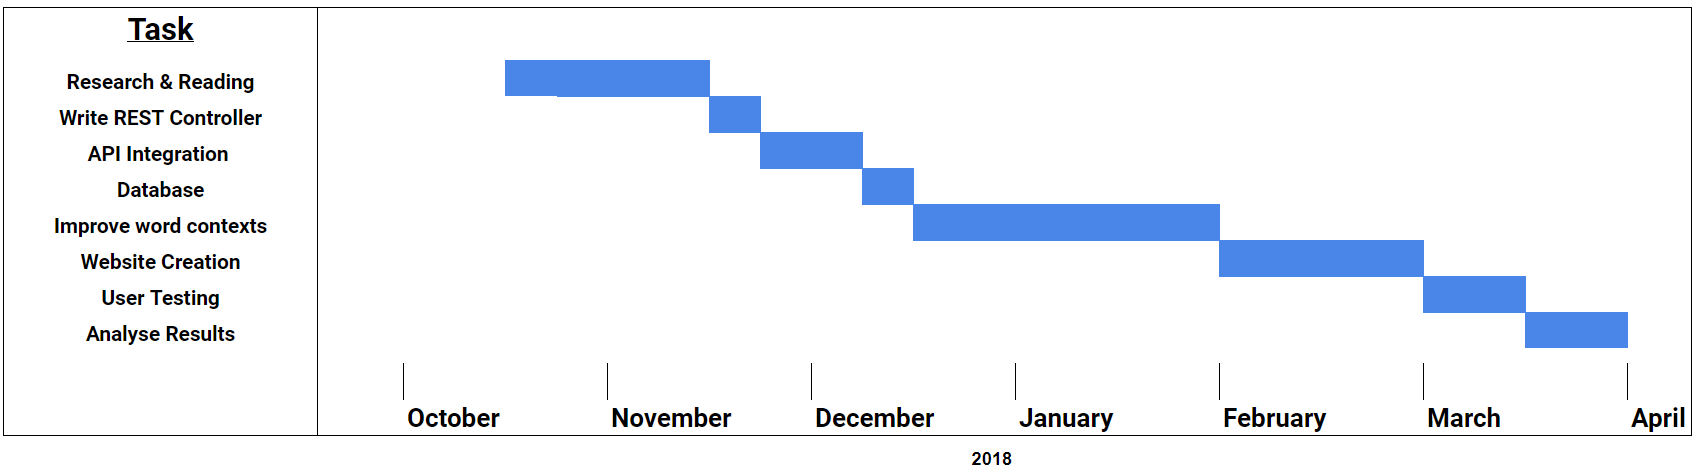
\includegraphics[scale=0.45]{gantt.png}}
\newline

Progress thus far has gone to plan. Most of the boilerplate code for the Back-end is completed, for which the estimated completion date was mid December. This work includes creating a Mongo database which can store user information, as well as integrating Oxford Dictionary API to the REST controller. \\

My sole focus for this month (December) will be the creation and implementation of the sentence-sorting algorithm --- which was labelled as `Improve word contexts' on the original work plan. Since progress is going according to plan, the only changes required for the work plan are the re-naming of tasks: \\

\noindent
\makebox[\textwidth]{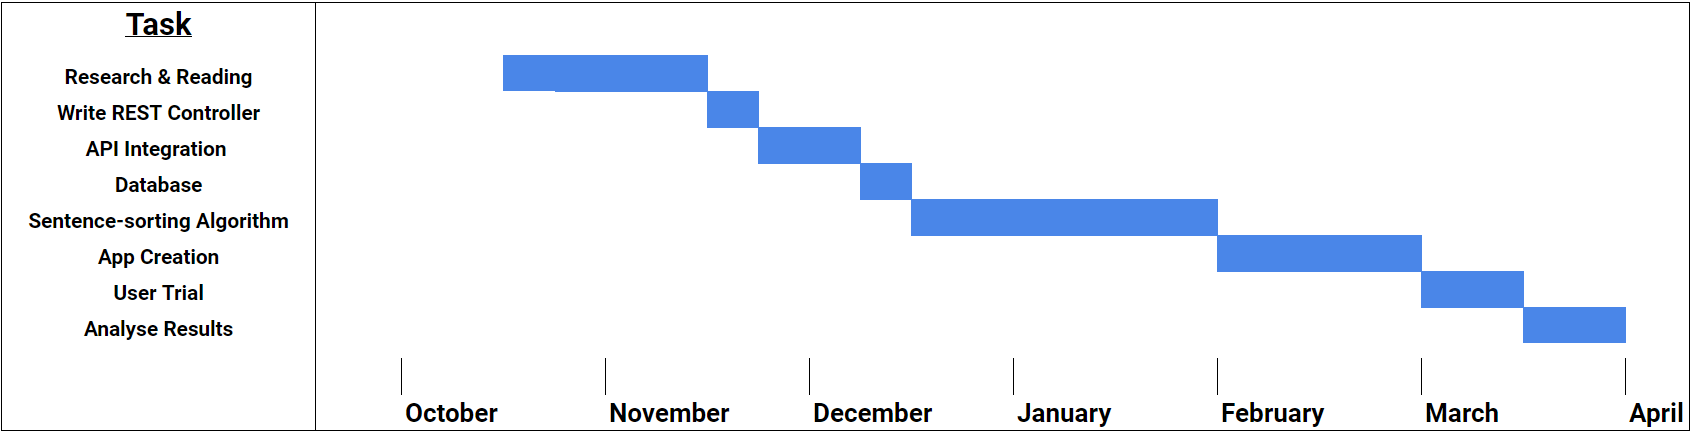
\includegraphics[scale=0.45]{gantt2.png}}
\newline

\subsection{Rules for `useful' sentences}

This list of rules is likely to change in the next month, but here are the rules I have denoted thus far --- largely as a result of my `Research \& Reading' task. 

\begin{enumerate}
\item The sentence must contain contextual information about the word in question. This contextual information is likely to take the form of a word association. For example, the word `coffee’ has an association with the word `hot’. 
\item It is preferable if this contextual information occurs before the word in question. The experiment run by (\cite{swinney1979lexical}) showed the importance of previous context in the recognition process. 
\item The key `association’ words must be relatively known words. ``To guess successfully from context, a reader must know the majority of the other words in that context.’' (\cite{schmitt1997vocabulary}). It is no use providing clues which don’t make sense to the user. In order to prevent this from happening, the algorithm will have to check for the word frequencies of the word in question.
\item ``Clues nearer the unknown word are easier to use than clues further away.’' (\cite{schmitt1997vocabulary}).
\end{enumerate}

\section{Considerations}
\subsection{Possibility of multi-language support}
One objective I have --- time providing --- is to offer support for different languages. This would create a new use case and appeal to a wider variety of learners. It is useful to know how many words in a language one needs to know in order to gain proficiency. (\cite{university1956study}) found that knowing just 2000 words can contribute to a 96\% understanding of informal spoken language. This data is useful because MyWords will include a statistics page which will show the user how many words they have learnt. This means that the user will be able to track their progress and be notified when they reach a stage that suggests a good level of proficiency. This sense of progress and achievement could encourage people to learn even more words. It would be helpful to obtain a list of the 2000 most frequently used words for each language that is supported. Using these lists, MyWords could offer suggestions as to which words user’s should prioritise. \\

Deciding on which list to use isn't straight forward, namely because there is a significant difference between spoken language and written language. (\cite{stenstrom1990lexical}) discusses the words that are more prevalent in the spoken form than written. For example, the word `just’ is used two and a half times more frequently in spoken language than written. Considerations need to be made as to which set of words should be more important. The ideal solution may be to use word lists for both spoken and written language. The user could then be offered a choice based on how they intend to use the language in question. One one hand, a user going on holiday to France probably only needs to be able to make conversation, and would be less concerned with understanding of books and text. On the other hand, a user intending to emigrate to France would be required to have a solid understanding of the language’s written form.

\subsection{Issue of Multiple Meanings}

Words tend to have multiple meanings, or \emph{senses}. When taking the most common 121 nouns and 70 verbs in the WordNet dataset, there were found to be an average of 7.8 senses per noun, and 12 per verb (\cite{ng1996integrating}). This creates a potential conflict in the quest to find good example sentences. Namely, there is the challenge of interpreting which meaning the user is trying to learn when they query a word. A simple solution would be to allow the user to choose the specific meaning that they want to learn and be tested on. This would entail the user clicking on one of the senses returned by the Oxford Dictionary API. \\

However, this approach would offer a new set of problems. If the application were to rely on Oxford’s data to interpret which meaning the user wants, the only example sentences readily available would be those provided by Oxford for that particular meaning. Consider the verb `run’ as an example. This word can be used in the context of `running a marathon’ or `running for president’. The Oxford Dictionary API will provide a number of example sentences for each of these senses. But if I were to try to find example sentences containing `running’ from elsewhere, I would face the task of having to interpret which sense of `running’ the sentence is conveying. This would not be trivial and it will be decided soon whether or not this is the correct direction to go. \\

The alternative is to obtain one set of sentences for each word, without regarding the various usages. The algorithm would then prioritise the frequently-used senses (because there would naturally be more examples of such usages). The advantage of this approach is that it greatly increases the number of sentences I could input to the sentence-sorting algorithm. This means that I could use text from the vast number of open-source ebooks available online. The disadvantage of this approach is that it could mean that the user will be quizzed on a meaning of a word that they didn’t intend to learn. (\cite{baicheng2009})

\subsection{The importance of repeated exposures}

There are several estimates for the difficult question: `How many exposures are required to learn a word?’
(\cite{Nation1990}) suggested that one needs to receive 5-16 exposures of the word in order to learn it. Regardless of what the true figure is, it seems that `numerous exposures’ is a criterion for the successful acquisition and retention of a word. MyWords needs to satisfy this need in order to achieve its goal. The quiz experience will offer some repeated exposure but nowhere near the 5-16 threshold.\\

The user will get the chance to gain these exposures from a `MyWords’ page which will show them their most recent queried words. This page will show them the definition of the word as well as some example sentences. I would also like this page to show any example sentences created by the user themselves. (\cite{baicheng2009}) found that students were more likely to remember a given word if they,  themselves wrote an example sentence for the word, rather than being handed one. The evidence for this is fairly limited however it is very much in line with the `Levels of Processing Hypothesis’. Since the user spends more cognitive energy on the word, the word will become easier to recall. The user will be encouraged to make the sentence as personal as possible.  







